\chapter{Umsetzung}
Dieses Kapitel erläutert alle Schritte der Umsetzung des GuttenBase Plugins beginnend mit der Analyse bis zu zur Architektur und Implementierung.
\section{Analyse}
Am Anfang dieses Abschnitts wird die Umsetzungsform des GuttenBase Plugins festgelegt, da diese einen Einfluss auf die Architektur sowie die zu verwendenen Technologien hat. Außerdem werden die Anforderungen an das System definiert.\\
Um den Soll-Zustand genauer zu definieren werden Prototypen eingesetzt.
\subsection{Umsetzungsform}
Um eine optimale Nutzung des GuttenBase Plugins zu erzielen, soll auf die Umsetzungsform geachtet werden.\\
Das zu entwickelnde Tool kann z. B. als eine Desktop Applikation, Web Applikation oder als Plugin einer anderen Anwendung realisiert werden.\\
In der Tabelle \ref{table:tool-options} werden einige Vor- und Nachteie jeder Alternative erläutert. \\
Alle drei Alternativen haben Pros und Contras allerdings ist die schnellere Erreichung von vielen Nutzern sowie die Einfache Installation bei der IDE Plugin Entwicklung entscheidend. 
\begin{table}
	\centering
		\begin{tabular}{ |p{3cm}|p{6cm}|p{6cm}| }
			\hline
			\textbf{Alternative} & \textbf{Vorteile} &  \textbf{Nachteile}  \\
			Desktop App & 
			\begin{itemize}
				\item Offline immer verfügbar
				\item Volle Kontrolle über die Anwendung und die enthaltenen Daten.
				\item Bessere Leistung, da kein Browser als Zwischenschicht existiert.
			\end{itemize}& 
			\begin{itemize}
				\item Platformabhängig
				\item Hohe Entwicklungskosten
				\item Installation ist notwendig
			\end{itemize} \\
			\hline
			Web App &
			
			\begin{itemize}
				\item Installation oder manuelle Updates sind nicht notwändig. 
				\item geringere Entwicklung- und Wartungskosen, da die Anwendung unabhängig von lokalen Endgeräten ist.
			\end{itemize} &
		
			\begin{itemize}
				\item Offline meistens nicht verfügbar.
				\item Geringere Leistung.
				\item Es kann auf bestimmte Gerätehardware nicht zugegriffen werden.
			\end{itemize} \\
			\hline
			IDE Plugin Entwicklung &
			
			\begin{itemize}
				\item Viele Nutzer können erreicht werden.
				\item Einfach zu installieren.
				\item Manche Komponenten bzw. Funktionalitäten der zu erweiternden IDE können wiederverwwendet werden, was die Entwicklungsdauer verkürzt.
				\item Intuitive Nutzung sowie eine einheitliche Benutzeroberfläche wie die benutzte IDE.
			\end{itemize} &
			
			\begin{itemize}
				\item Einarbeitung in die Plugin Entwicklung der ausgewählten IDE ist erforderlich.
				\item Die Flexibilität beim Entwickeln ist durch die limitierte Erweiterbarkeit der IDE eingeschränkt.
			\end{itemize} \\
			\hline
		
		\end{tabular}
	\caption{Umsetzungsmöglichkeiten}
	\label{table:tool-options}
\end{table}

Zunächst soll für eine konkrete IDE entschieden werden. Um diese auszuwählen, muss auf die Anzahl der Nutzer, die Verfügbarkeit der Dokumentation für Plugin Entwicklung sowie die Unterstützung von Datenbanken geachtet werden.\\
Einer der bekanntesten Methoden, um die Beliebtheit einer Programmiersprache bzw. eine IDE herauszufinden, ist der PYPL-Index. Er basiert sich auf Rohdaten aus Google Trends. PYPL enthält den TOP-IDE-Index, welches alanysiert, wie oft IDEs bei Google durchgesucht werden. Die Suchanfragen spiegeln zwar nicht unbedingt die Beliebtheit der IDEs spiegeln. Allerdings hilft einen solchen Index bei der Wahl einer Entwicklungsumgebung.
Bei dieser Analyse sind die drei bekanntesten und für unseren Fall relevanten Entwicklungsumgebungen Visual Studio (erster Platz), Ecllipse (zweiter Platz) und IntelliJ (sechster Platz). Außerdem hat sich der Index von IntelliJ IDE am stärksten erhöht (siehe Abbildung \ref{img:ide-index})\\
Bei eine anderen Umfrage (Jaxenter), mit welcher Entwicklungsumgebung am liebsten in Java programmiert wird, war IntelliJ sogar im ersten Platz mit 1660 Stimmen von 2934. \\

\begin{figure}[h]
	\caption{Top IDE Index}
	\centering
	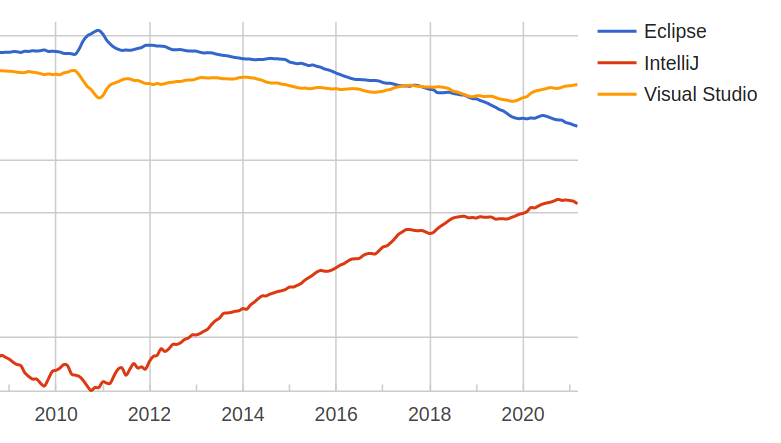
\includegraphics[width=0.8\textwidth]{images/ide-index}
	\label{img:ide-index}
\end{figure}
Aus den oben fgenannten Gründen wird das GuttenBase als ein Intellij Plugin umgesetzt werden. 

\subsection{Allgemeine Beschreibung der Anforderungen}
Die Anforderungsanalyse ergab folgende Punkte, die von dem GuttenBase Plugin erfüllt werden sollen:
\begin{enumerate}
	\item \textbf{Konfigurationsschritte verwalten:}\\
	Um den Migrationsprozess zu individualisieren, soll der Benutzer die Möglichkeit haben, neue Konfigurationsschritte zu erstellen, zu editieren und zu löschen.
	\item \textbf{Konfigurationsschritte speichern:} \\
	hinugefügte Konfigurationsschritte sollen nach Bestätigung vom Benutzer gespeichert werden können. Diese sollen auch nach einem Neustart der Anwendung zur Verfügen stehen.
	\item \textbf{Überblick über alle Konsfigurationsschritte:}
	Der Benutzer soll über eine tabellarische Auflistung aller erstellten Konfigurationsschritte haben.
	\item \textbf{Datenbanken Verbiden:} \\
	Um eine erfolgreiche Migration durchzuführen, soll der Benutzer in der Lage sein, eine Verbindung zwischen der Quell- und Ziel-Datenbank herzustellen. Die zu migrierende Datenbank sowie die Ziel-Datenbank sollen aus den existierenden Datenbanken ausgewählt werden können.
	\item \textbf{Überblick über enthaltene Datenbankelemente:}\\
	Während des Pigrationsprozess, soll der Benutzer einen Überblick über alle in der Quell-Datenbank enthaltenen Tabellen bzw. Spalten verfügen.
	\item \textbf{Existierende Konfigurationsschritte zur Migration hinzufügen:}\\
	Gespeicherte Konfigurationsschritte sollen bei der Übersicht der Datenbank Elementen zur Verfügung stehen. Diese können auf die entsprechenden Datenbank Elementen angewendet werden.
	\item \textbf{Hinzugefügte Konfigurationsschritte löschen:}\\	
	Der Benutzer soll die Möglichkeit haben, hinzugefügte Konfigurationsschritte zu löschen, nachdem sie zur Migration hinzugefügt wurden.
	\item \textbf{Migrationssprozess starten:} \\
	Im letzten Schritt der Migration kann der Benutzer den Migrationsprozess mit den hinzugefügten Konfigurationsschritten starten.	
	\item \textbf{Überblick über den Fortschritt der Migrationsprozess:}\\
	Damit der Benutzer den Migrationsprozess verfolgen kann, soll einen Überblick über den Fortschritt zur verfügung stehen. 
\end{enumerate}
Konfigurationsschritte beziehen sich hauptsächlich auf die Hinweise der GuttenBase Bibliothek. Um den Umfang dieser Arbeit in Grenzen zu halten, wurden folgende wichtige Konfigurationsschritte für die Umsetzung ausgewählt:

\begin{enumerate}
	\item Spalten  umbenennen.
	\item Tabellen umbenennen.
	\item Filteroptionen für Spalten hinzufügen.
	\item Filteroptionen für Tabellen hinzufügen.
	\item Datentypen von Spalten ändern.
\end{enumerate}

\subsection{detaillierte Beschreibung der Anforderungen}
Dieser Abschnitt beschäftigt sich mit den zu implementierenden Anforderungen. Diese decken den wichtigsten Funktionsumfang des Systems.\\
Neben der textuellen Beschreibung werden auch Anwendungsfalldiagramme erstellt. Dabei wird nur ein Akteur identifiziert. Dieser ist der Benutzer, der die Datenbank Migration durchführt.
\subsubsection{Konfigurationsschritt \textbf{Unbenennen} hinzufügen}
Dieser Anwendungsfall bildet den Vorgang ab, wenn ein Benutzer einen neuen Konfigurationsschritt für das Umbenennen von Spalten bzw. Tabellen in der Ziel-Datenbank. Dies passiert nachdem der Benutzer die Option Umbenennen auswählt und dann
\subsubsection{Konfigurationsschritt \textbf{Excludieren} hinzufügen}
\subsubsection{Konfigurationsschritt \textbf{Spaltentypen Ändern} hinzufügen}
\subsubsection{Konfigurationsschritte verwalten}
\subsubsection{Datenbank Migration durchführen}

\subsection{Prototypen}
%\subsection{Probleme und Strategien}
%- Umsetzungsform\\
%- ...
\section{Konzeption}
%- DatenModell: GBActions, DB Elemente\\
%- Abstrakte Mapping \\
%- Multiple Select \\
%- Aktionen speichern \\
%- Protoypen \\
%- allgemeines: warum muss erst die Umsetzungsform entschieden werden (vor der Konzeption). \\
%- welche Alternativen gibt es um ein solches Plugin entwickeln zu können?\\
%- Vorteile und Nachteile jeder Alternative.\\
%- Argumente für IntelliJ Plugin.
%- Was ist IntelliJ \\
%- was ist IntelliJ Plugin Entwicklung \\
%- wie lässt sich ein Plugin mit IntelliJ entwickeln?\\

\subsection{Anwendungsfälle}
\subsection{Konzeptionelle Sicht}
\subsection{Modulsicht}
\subsection{Datensicht}



\section{Implementierung}
\subsection{verwendete Technologien}
- Swing \\
- UI Form \\
- Java\\
- Gutenbase
\subsubsection{IntelliJ Plugin Entwicklung}

\subsection{Features}
%- add gbact\\
%- save gb act\\
%- migrate db \\
%- + screenshots usw.


